%%%%%%%%%%%%%%%%%%%%%%%%%%%%%%%%%%%%%%%%%%%%%%%%%%%%%%%%%%%%%%%%%%%%%%%%%%%%%%%%
%%%%%%%%%%%%%%%%%%   Vorlage für eine Abschlussarbeit   %%%%%%%%%%%%%%%%%%%%%%%%
%%%%%%%%%%%%%%%%%%%%%%%%%%%%%%%%%%%%%%%%%%%%%%%%%%%%%%%%%%%%%%%%%%%%%%%%%%%%%%%%

% Erstellt von Maximilian Nöthe, <maximilian.noethe@tu-dortmund.de>
% ausgelegt für lualatex und Biblatex mit biber

% Kompilieren mit
% lualatex dateiname.tex
% biber dateiname.bcf
% lualatex dateiname.tex
% lualatex dateiname.tex
% oder einfach mit:
% make

\documentclass[
  tucolor,
  BCOR=12mm,     % 12mm binding corrections, adjust to fit your binding
  parskip=half,  % new paragraphs start with half line vertical space
  open=any,      % chapters start on both odd and even pages
  cleardoublepage=plain,  % no header/footer on blank pages
]{tudothesis}

% \usepackage{geometry}
% \geometry{a4paper, margin=2.5cm, top=3.5cm}
% \usepackage[onehalfspacing]{setspace}

% Warning, if another latex run is needed
\usepackage[aux]{rerunfilecheck}

% just list chapters and sections in the toc, not subsections or smaller
\setcounter{tocdepth}{1}

%------------------------------------------------------------------------------
%------------------------------ Sprache und Schrift: --------------------------
%------------------------------------------------------------------------------
\usepackage{fontspec}
\defaultfontfeatures{Ligatures=TeX}  % -- becomes en-dash etc.

% german language
\usepackage{polyglossia}
\setdefaultlanguage{english}

% for german parts if needed
\setotherlanguages{german}

% intelligent quotation marks, language and nesting sensitive
\usepackage[autostyle]{csquotes}

% microtypographical features, makes the text look nicer on the small scale
\usepackage{microtype}

%------------------------------------------------------------------------------
%------------------------ Für die Matheumgebung--------------------------------
%------------------------------------------------------------------------------

\usepackage{amsmath}
\usepackage{amssymb}
\usepackage{mathtools}

% Enable Unicode-Math and follow the ISO-Standards for typesetting math
\usepackage[
  math-style=ISO,
  bold-style=ISO,
  sans-style=italic,
  nabla=upright,
  partial=upright,
]{unicode-math}
\setmathfont{Latin Modern Math}

% nice, small fracs for the text with \sfrac{}{}
\usepackage{xfrac}


%------------------------------------------------------------------------------
%---------------------------- Numbers and Units -------------------------------
%------------------------------------------------------------------------------

\usepackage[
  locale=DE,
  separate-uncertainty=true,
  per-mode=symbol-or-fraction,
]{siunitx}
\sisetup{math-micro=\text{µ},text-micro=µ}

%------------------------------------------------------------------------------
%-------------------------------- tables  -------------------------------------
%------------------------------------------------------------------------------

\usepackage{booktabs}       % stellt \toprule, \midrule, \bottomrule

%------------------------------------------------------------------------------
%-------------------------------- graphics -------------------------------------
%------------------------------------------------------------------------------

\usepackage{graphicx}
\usepackage{grffile}
\usepackage{subcaption}

% allow figures to be placed in the running text by default:
\usepackage{scrhack}
\usepackage{float}
\floatplacement{figure}{htbp}
\floatplacement{table}{htbp}

% keep figures and tables in the section
\usepackage[section, below]{placeins}


%------------------------------------------------------------------------------
%---------------------- customize list environments ---------------------------
%------------------------------------------------------------------------------

\usepackage{enumitem}

%------------------------------------------------------------------------------
%------------------------------ Bibliographie ---------------------------------
%------------------------------------------------------------------------------

\usepackage[
  backend=biber,   % use modern biber backend
  autolang=hyphen, % load hyphenation rules for if language of bibentry is not
                   % german, has to be loaded with \setotherlanguages
                   % in the references.bib use langid={en} for english sources
]{biblatex}
\addbibresource{references.bib}  % die Bibliographie einbinden
\DefineBibliographyStrings{german}{andothers = {{et\,al\adddot}}}

\usepackage[labelformat=simple]{subcaption}
\renewcommand\thesubfigure{(\alph{subfigure})}

%------------------------------------------------------------------------------
%------------------------------ Sonstiges: ------------------------------------
%------------------------------------------------------------------------------

\usepackage[pdfusetitle,unicode,linkbordercolor=tugreen]{hyperref}
\usepackage{bookmark}
\usepackage[shortcuts]{extdash}

%------------------------------------------------------------------------------
%-------------------------    Angaben zur Arbeit   ----------------------------
%------------------------------------------------------------------------------

\author{Kevin Sedlaczek}
\title{Analysis of the Crab Nebula using Photon Stream data collected by FACT}
\date{\today}
\birthplace{Dortmund}
\chair{Lehrstuhl für Experimentelle Physik Vb}
\division{Fakultät Physik}
\thesisclass{Arbeit zur Erlangung des akademischen Grades Master of Science}
\submissiondate{31. Dezember 2018}
\firstcorrector{Prof.~Dr.~Dr.~Wolfgang Rhode}
\secondcorrector{Prof.~Dr.~Zweitkorrekteur}

% tu logo on top of the titlepage
\titlehead{
\includegraphics[height=1.5cm]{logos/tu-logo.pdf}}

\begin{document}
\frontmatter
% \input{content/hints.tex}
\maketitle

% Gutachterseite
\makecorrectorpage

% hier beginnt der Vorspann, nummeriert in römischen Zahlen
\chapter{Abstract}

This work is investigating the novel data format \textit{Photon Stream} by
analyzing physics data of the Crab Nebula. \textcolor{red}{Nicht vollständig}
\\
\\
In dieser Arbeit wird das neuartige Datenformat \textit{Photon Stream} im
Zusammhang einer Analyse des Krebsnebels untersucht.

\tableofcontents

\mainmatter
% Hier beginnt der Inhalt mit Seite 1 in arabischen Ziffern
\chapter{Introduction}
\nocite{biblatex, siunitx, Hunter:2007}%
%
\begin{aquote}{\textit{Albert Einstein}}
\textsc{One cannot help but be in awe when he contemplates the mysteries of eternity, of life, of the marvelous structure of reality.}
\end{aquote}
In physics, the search for a fundamental understanding of reality is ubiquitous. The understanding of the universe we live in and the rules of nature has
led mankind to look for the things beyond earth. To understand what these rules
are, on earth and in the universe, is the goal of astrophysics. The electromagnetic radiation reaching the earth from space has opened the window to learn
about the universe beyond our planet. The discovery of this extraterrestrial
radiation by Victor Hess during his balloon flights around \num{100} years ago in \num{1912}~\cite{Hess} marks the beginning of the observation of this radiation.
Today we know that the electromagnetic radiation spans a very large range of
frequencies and reaches up to the highest energies ever measured \cite{source}.
The different energy ranges of cosmic radiation caused the development of a
variety of different telescopes, specialized on certain frequency bands. On
ground, only visible light and radio waves from space can be observed directly,
due to the absorption of Earth's atmosphere. Therefore, large optical and radio
telescopes have been built to observe stars, galaxies and other objects from
Earth. Of course, the atmosphere still has an impact on the observations, so
there are optical telescopes in space as well, like the Hubble Space
Telescope~\cite{hubble}, observing infra-red to ultra-violett light. However,
some telescopes take advantage of the atmosphere's impact, by using it as a
giant detector volume. Among these telescopes are the Imaging Air Cherenkov
Telescopes (IACT), observing cosmic rays via their interaction products. This
work is based on the observations of such a telescope, described in
\autoref{ch:fact}. The development and advancement of new telescopes continues
today, as the currently constructed Cherenkov Telescope Array CTA~\cite{cta}
will yield unprecedented accuracy and sensitivity among IACTs.
Among the goals of astrophysics are not only the understanding of the
structures of the universe, but also the very elementary interactions of
particles within the sources of this radiation. The very first hints for the
existance and characteristics of dark matter~\cite{zwicky}, a supposed
elementary particle for instance originate from the field of astrophysics.
This work focuses on the rather technical aspect of a new data representation
and its implications for IACT analyses, by analyzing a data set of this new data
format for the first time.

\chapter{Representing IACT data}

There are different ways to represent air shower data. FACT uses the so called main-pulse representation, whereas this work focuses on a novel data format, both of which are described in the following chapter.

\section{The Main-Pulse representation}
Data that has been taken by an Imaging-Air-Cherenkov-Telescope
(IACT), like FACT, is usually represented in so called time series.
These time series owe their name to the fact that they represent voltages at the photosensors over time. Within these time series lie so called main-pulses that represent the increased voltage that a charge deposition of an air shower causes. So by looking for those main-pulses shower events can be found upon the detector noise and ambient light in the camera. Of course, the main-pulses consist of multiple photon signals superposed over time, but they are first described by electric pulses. This means that the charge deposit has to be transferred into physics observables. By integrating the charge in one pixel and equivalent of a photon count can be obtained, called the \textit{photon equivalent} (PE). So the first observable in this representation is the PE which corresponds to the number of photons measured. The photon counts are spatially located by the corresponding pixel they are assigned to. The 1440 pixels of FACT are the determining grid that yield the spatial coordinates of every shower event. The last observable is the time. When the telescope is triggered and records data the arrival time of the photons is measured as explained above. From the time series a quantized timing information per pixel can be developed by dividing the event into time slices. Thus, the arrival times $t$ are the third observable of the main-pulse event representation.

\begin{figure}
  \centering
  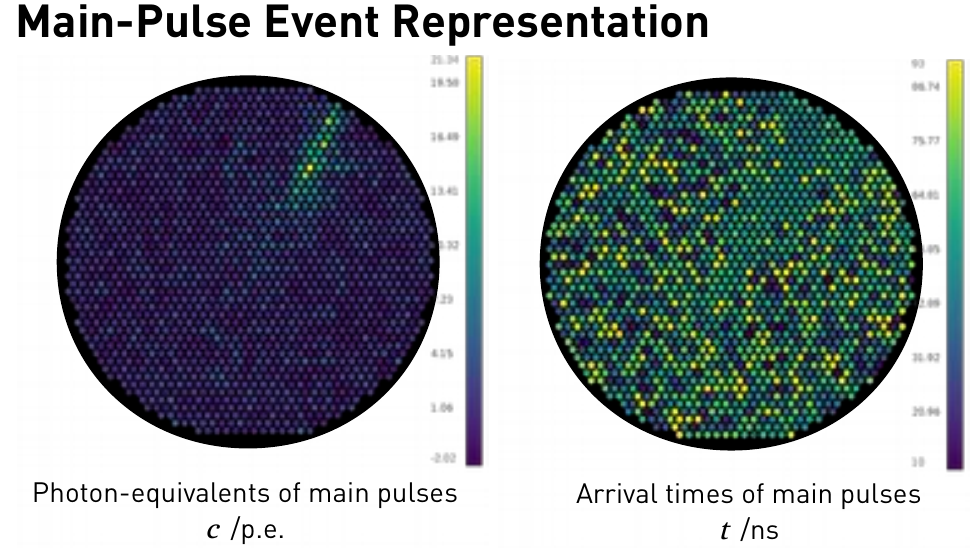
\includegraphics[width=0.7\textwidth]{Plots/standard.png}
  \caption{The measured observables of the main-pulse representation are shown as scatter plots within the pixels. On the left the distribution of photon equivalents $c$ of a typical shower event is shown as well as the arrival times of that events photons on the right.}
  \label{fig:mainpulse}
\end{figure}

\section{The Photonstream representation}

The Photonstream representation aims at creating a data format consisting of photons by storing their observed physical properties. So from the measured time series single photons are extracted instead of deriving photon counts in pixels. Each of these photons is assigned an arrival time and pixel, creating a list of arrival times per photon for each pixel. By doing so, a 3-dimensional data set is created, which can be represented in form of so called point clouds (\autoref{fig:event}).
%
\begin{figure}
  \begin{subfigure}{0.475\textwidth}
    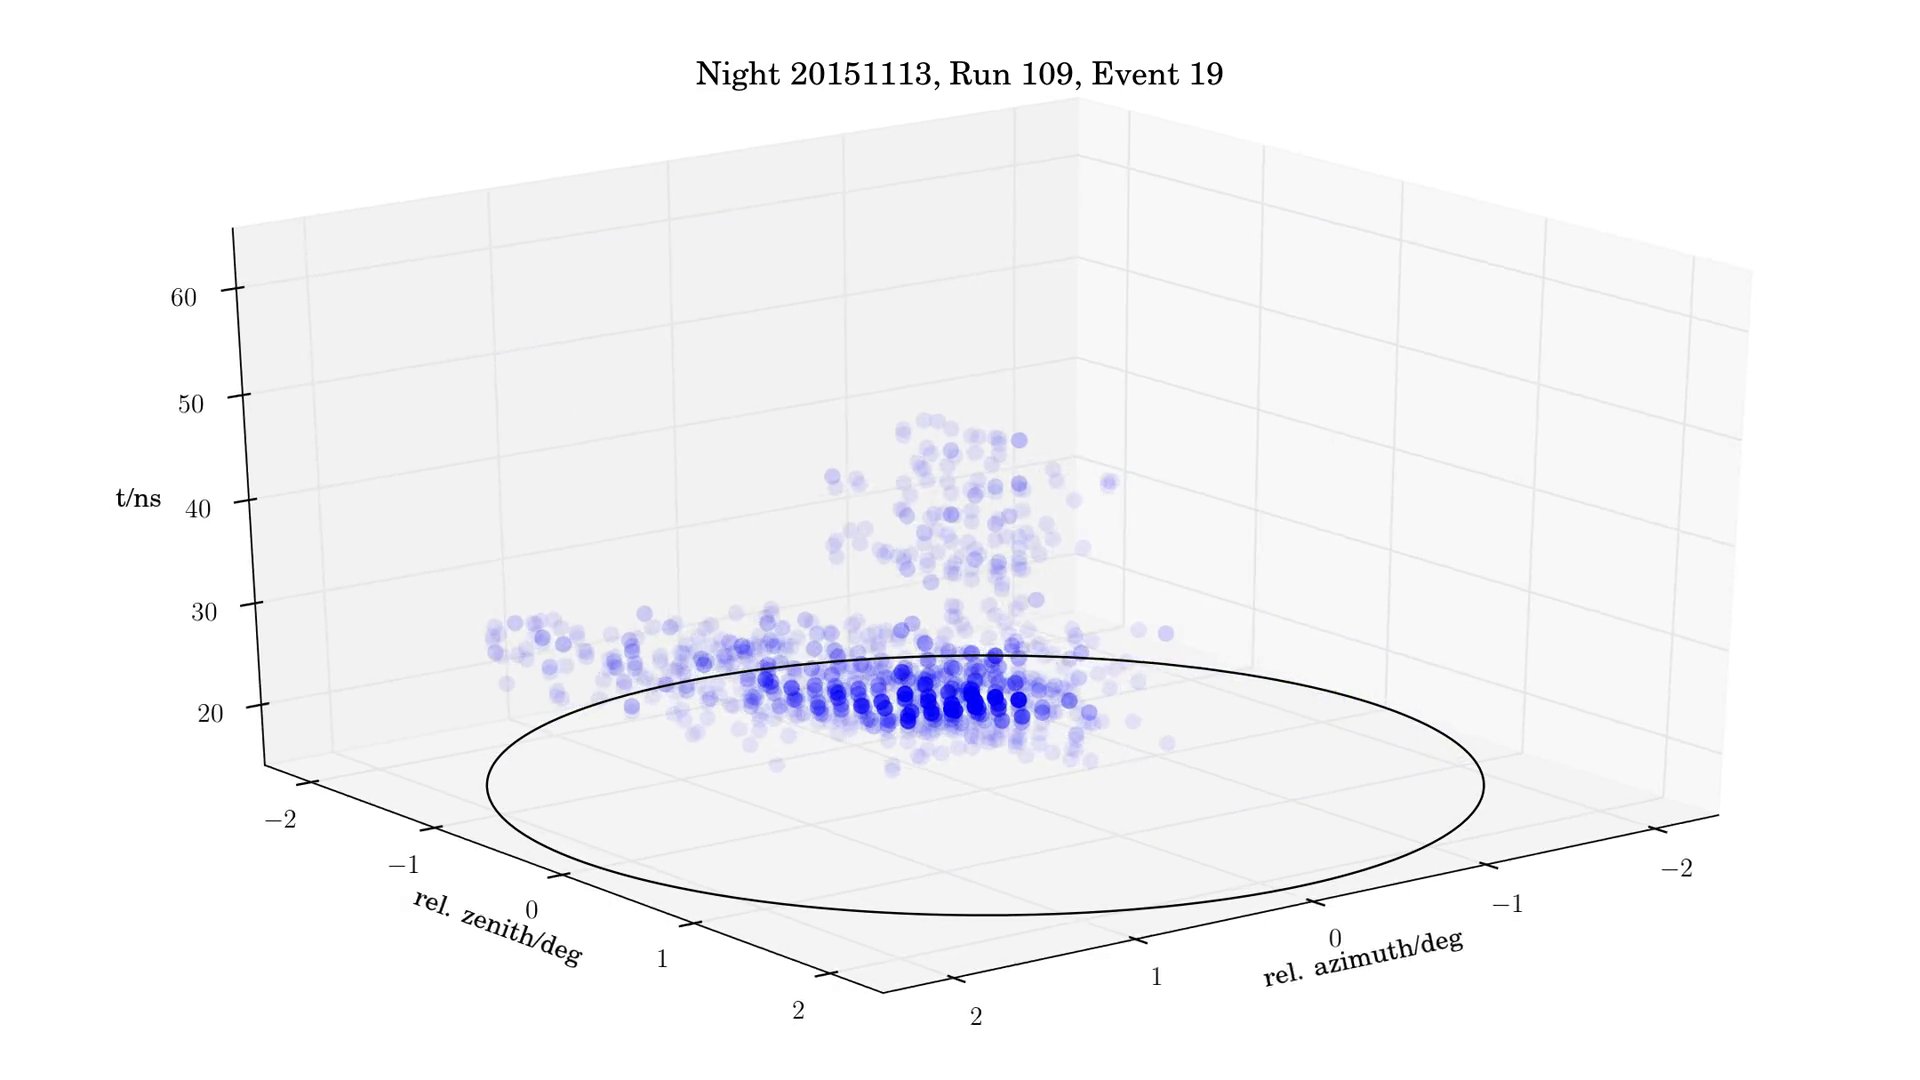
\includegraphics[width=1.1\textwidth]{Plots/event1.png}
  \end{subfigure}
  \begin{subfigure}{0.475\textwidth}
    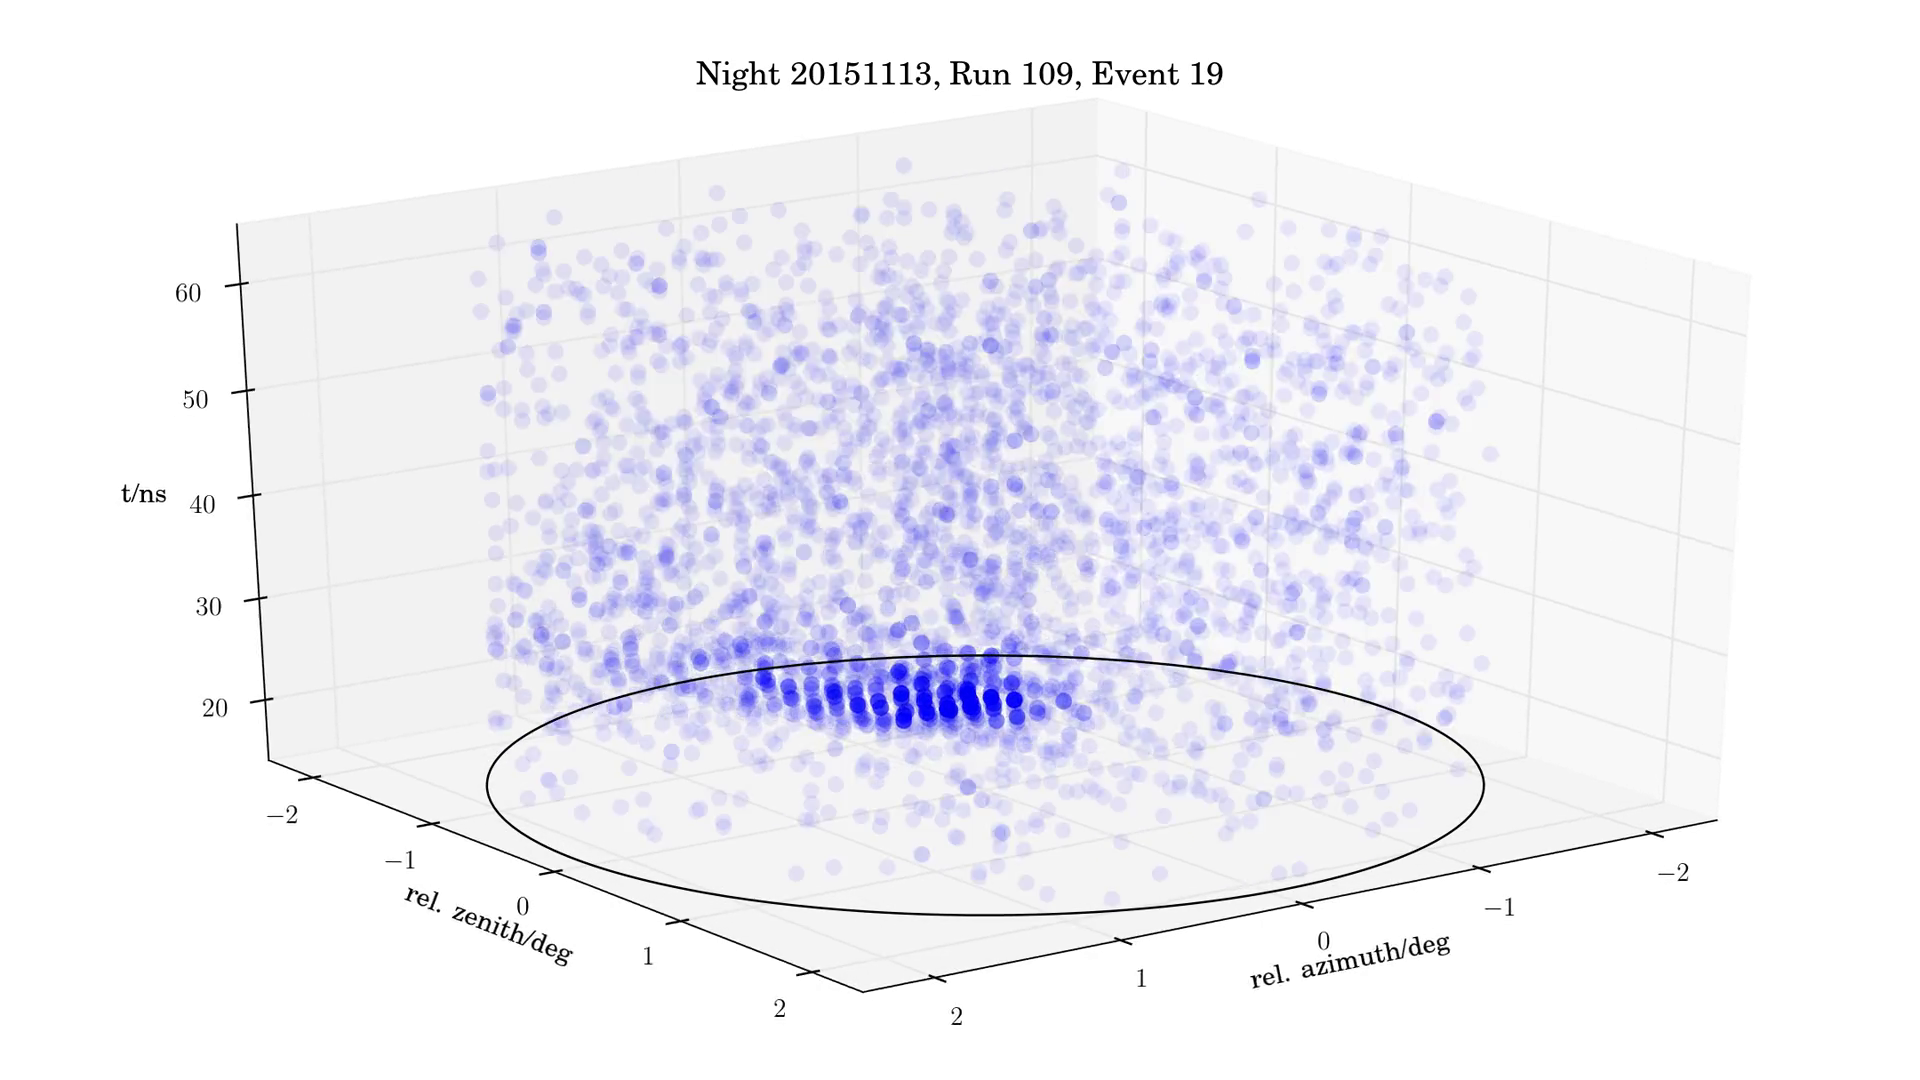
\includegraphics[width=1.1\textwidth]{Plots/event2.png}
  \end{subfigure}
  \caption{Event represented by the 3-dimensional point cloud of the Photonstream. Every blue sphere represents a measured photon in the corresponding time slice and pixel. The left figure shows the remaining photons after cleaning.}
  \label{fig:event}
\end{figure}

% \input{content/03_hauptmethode.tex}
% \input{content/04_alternative.tex}
% \input{content/05_results.tex}


\appendix
\clearpage
% Hier beginnt der Anhang, nummeriert in lateinischen Buchstaben
\chapter{Appendix A}

\begin{table}
  \centering%
  \begin{tabular}{l
                  c
                  c}
      \toprule
      {}    & Anzahl der Filter in den Dichtelagen  & Struktur der Dropout Lagen      \\
      \midrule
      Modell 0    & (1024, 512, 128, 64, 32)  & (0.5, 0.4, 0.4, 0.3, 0.2) \\
      Modell 1    & (1024, 512, 256, 128, 64, 32, 16)  & (0.5, 0.4, 0.4, 0.4, 0.2, 0.2, 0.1) \\
      Modell 2    & (512, 256, 128, 64, 32, 16)  & (0.4, 0.4, 0.3, 0.3, 0.2, 0.1) \\
      Modell 3    & (1024, 256, 64, 16)  & (0.6, 0.4, 0.2, 0.1) \\
      Modell 4    & (512, 128, 32)  & (0.5, 0.3, 0.1) \\
      \bottomrule
  \end{tabular}
  \caption{Getestete Grundstrukturen für die Netzarchitekturen der alternativen Methode. Das $n$-te Element der Tupel beschreibt jeweils die Filtergröße der $n$-ten Dichtelage. Selbiges gilt für die Dropout Lagen. Es folgt auf jede Dichtelage (abgesehen von der letzten Lage) eine Dropout Lage.}
  \label{tab:grid}
\end{table}
%


\backmatter
\printbibliography

\cleardoublepage
\thispagestyle{empty}
\section*{Eidesstattliche Versicherung}
Ich versichere hiermit an Eides statt, dass ich die vorliegende Abschlussarbeit mit dem Titel \enquote{\thetitle} selbstständig und ohne unzulässige fremde Hilfe erbracht habe.
Ich habe keine anderen als die angegebenen Quellen und Hilfsmittel benutzt, sowie wörtliche und sinngemäße Zitate kenntlich gemacht.
Die Arbeit hat in gleicher oder ähnlicher Form noch keiner Prüfungsbehörde vorgelegen.

\vspace*{1cm}\noindent
\begin{center}
  \begin{tabular}{@{}p{0.4\textwidth}@{\hspace{0.15\textwidth}}p{0.4\textwidth}@{}}
  \rule{\linewidth}{0.25pt}& \rule{\linewidth}{0.25pt}\\
  Ort, Datum & Unterschrift
  \end{tabular}
\end{center}

\subsection*{Belehrung}
Wer vorsätzlich gegen eine die Täuschung über Prüfungsleistungen betreffende Regelung einer Hochschulprüfungsordnung verstößt, handelt ordnungswidrig.
Die Ordnungswidrigkeit kann mit einer Geldbuße von bis zu \SI[round-mode=places, round-precision=2]{50000}{€} geahndet werden.
Zuständige Verwaltungsbehörde für die Verfolgung und Ahndung von Ordnungswidrigkeiten ist der Kanzler/die Kanzlerin der Technischen Universität Dortmund.

Im Falle eines mehrfachen oder sonstigen schwerwiegenden Täuschungsversuches kann der Prüfling zudem exmatrikuliert werden \mbox{(\S\,63 Abs. 5 Hochschulgesetz --HG--).}

Die Abgabe einer falschen Versicherung an Eides statt wird mit Freiheitsstrafe bis zu 3 Jahren oder mit Geldstrafe bestraft.

Die Technische Universität Dortmund wird ggf.\ elektronische Vergleichswerkzeuge (wie z.\,B.\ die Software \enquote{turnitin}) zur Überprüfung von Ordnungswidrigkeiten in Prüfungsverfahren nutzen. \\[\baselineskip]

\noindent Die oben stehende Belehrung habe ich zur Kenntnis genommen.\\[1cm]
\begin{center}
\begin{tabular}{@{}p{0.4\textwidth}@{\hspace{0.15\textwidth}}p{0.4\textwidth}@{}}
\rule{\linewidth}{0.25pt}& \rule{\linewidth}{0.25pt}\\
Ort, Datum & Unterschrift
\end{tabular}
\end{center}

\end{document}
